\documentclass{article}
\usepackage{amsmath,amssymb,bbm, url,color}
\usepackage[hidelinks]{hyperref}
\usepackage{graphicx}

\addtolength{\textwidth}{2cm}
\addtolength{\hoffset}{-1cm}
\addtolength{\textheight}{2cm}
\addtolength{\voffset}{-1cm}

\newcommand{\mc}{\mathcal}
\DeclareMathOperator*{\argmax}{arg \, max}


\begin{document}
\title{
{\normalsize Lab sessions for the class}\\[-1mm]
Distributed Algorithms and Network Systems\\[-1mm]
{\normalsize MiSCIT Master -- Grenoble -- fall 2017}\\[-1mm]
{\normalsize prepared by Federica Garin, Ga\"{e}tan Harter, and Olivier Fambon}}
\date{}
\maketitle
%\vspace{-2cm}



\section{About this lab and the report}
In this lab, you will put in practice some distributed algorithms seen in class.
You will use the experimental platform FIT/IoT-lab (\url{https://www.iot-lab.info})
to execute your algorithms on real microcontrollers communicating through radio.\\

You are required to write a report, which will be graded.\\ Send it by e-mail to \texttt{federica.garin@inria.fr}.\\
Deadline: Wednesday, Nov.~1st.\\

Recommendations for a good report:
\begin{itemize}
\item Make sure to follow the instructions given in this document, and include all required items.
\item Write in clear English and precise math. Justify and explain all your statements, but be concise.
\item Figures require a caption. Plots require axes labels and legend.
\item Please include in the report a copy-paste of the relevant lines of C code that you have written.
\end{itemize}

\newpage

\section{Get familiar with FIT/IoT-lab}


\textit{\color{blue} This preliminary task is not meant to be described in your report. Just write a very short introduction (few lines!), stating the goal of this lab and mentioning the use of FIT/IoT-lab}\\


To familiarize yourself with the use of the platform:
\begin{itemize}
\item Read the testbed presentation at: \url{https://www.iot-lab.info/what-is-iot-lab/}
\end{itemize}

% OLD (2016)
%%%Then go to the page of tutorials and the following four tutorials (First steps):
%%%\begin{center} \url{https://www.iot-lab.info/tutorials/} \end{center}
%%%\begin{itemize}
%%%\item Configure your SSH access;
%%%\item Submit an experiment with Web portal: M3 nodes;
%%%\item Get and compile a firmware code for a M3 node.
%%%\item Tools$\to$Node-cli client (Update firmware from command line)
%%%\end{itemize}

Then go to the page of tutorials and the following four tutorials (First steps):
\begin{center} \url{https://www.iot-lab.info/tutorials/} \end{center}
\begin{enumerate}
   \item SSH access (Configure IoT-LAB access): \\
   \url{https://www.iot-lab.info/tutorials/configure-your-ssh-access/}
   \item M3 nodes (Submit and experiment with web portal): \\
   \url{https://www.iot-lab.info/tutorials/submit-an-experiment-with-web-portal-and-m3-nodes/}
   \item Build M3 and A8-M3 firmware (Compile firmware code for IoT-LAB)\\
   \url{https://www.iot-lab.info/tutorials/get-compile-a-m3-firmware-code/}
   \item Tools $\to$ Node -- cli client (Update firmware from command line) \\
   \url{https://www.iot-lab.info/tutorials/node-cli-client/}
\end{enumerate}

Make sure you have completed all tutorials before proceeding.




\section{Provided files and how to use them}

For this lab, you are given
an already-written firmware that allows you to interact with the nodes,
either in synchronous or gossip mode.
You will start by using the synchronous mode,
where there is a global notion of discrete-time iterations: at each iteration,
all communications take place, then all local computations are done.

In gossip mode (more precisely, this is a broadcast gossip), each node has a local Poisson clock; when a node is activated by its Poisson clock, it sends its state to its neighbors; all neighbors having received such message immediately proceed to do a local computation and update local state.


There are python scripts already written for you; the thing you will need to do
is to open some C file and modify it, so as to write the suitable functions for
the required computations.

\subsection{Accessing files on the server}

To simplify usage compared to what you did in the tutorial, a symbolic link has been
created in your home directory on the server \verb=~/distributed_algorithm=.
Everything can be done from this directory.\\


You should:
\begin{itemize}
\item Open a terminal, use \verb=ssh= to connect to your account and \\
    use \verb=cd= to change to \verb=distributed_algorithm= directory:
    \begin{verbatim}your_computer:$ ssh miscitXX@grenoble.iot-lab.info
miscitXX@grenoble:~$ cd ~/distributed_algorithm
miscitXX@grenoble:~/distributed_algorithm$
\end{verbatim}
This is where the files are sitting, that can be modified by you.

\item Use \verb=ls= to see which files are there. The ones you need are the following:
	\begin{itemize}
	\item You will need to modify \verb=computing.c= and \verb=clock_convergence.c= to add the functions for computing (more details below)
	\item In the file \verb=config.h=, you will need to modify:
		\begin{itemize}
%        \item The number of values (i.e., how many scalars there are in the state
%            of each node). This is the constant \verb=NUM_VALUES= defined
%            quite at the beginning of the file. You will need $1$ when doing
%            scalar consensus, you will need more when doing max-consensus
%            for node-counting. Choose an integer between $1$ and $14$.

		\item The channel: to avoid interfering with other groups, set the
            constant \verb=CHANNEL= to different numbers, group $x$ will take
            channel $10+x$, e.g., group 2 gets channel $12$
		\item Possibly, you might  need to modify another thing in this file:
            the power reception threshold \verb=MIN_RSSI= in case the graph is
            too sparse (disconnected) or too dense (too many communications, not
            an interesting example of distributed computing).\\
            The Received Signal Strength Indicator is in dBm, and there is a minus sign before the value,
            so putting a higher number means decreasing strength.
            Use values between -90dBm (noise level) and -55dBm (max RSSI).
         \item Some parameters of the local system clocks (to be used in the clock-synchronization exercice): \verb=TIME_SCALE=, \verb=TIME_SCALE_RANDOM=, and \verb=TIME_OFFSET_RANDOM=.
		\end{itemize}
    \item A \verb=subject= directory with \LaTeX~sources of the document that you are now reading.
    \item A \verb=results= directory to put all exercices intermediate results.
	\end{itemize}
\end{itemize}

You can open and modify the files directly on the server, without downloading
them to your local computer, just use \verb=nano <filename>.c= to open a file in
a text editor (to save the file after having modified it, follow instructions to
quit and then you will be prompted with the question where you wish to save it
(\verb=Ctrl+x= and \verb='O'=))


\subsection{Source file function description}


\subsubsection{Consensus: computing.c}

You will use \verb=computing.c= file for synchronous and broadcast-gossip consensuses.
The following function are of your interest:

\begin{itemize}
	\item  \verb=init_value()= does random initialization; this is for a scalar value.
%        It is called multiple times if \verb=NUM_VALUES=$\ge 2$ (remember,
%        this parameter is set in the file \verb=config.h=)
	\item \verb=compute_value_from_neighbours= has to be used only in the synchronous mode.\\
        It allows a node to compute its new state given: its own old state (\verb=my_value=),
        its own degree (\verb=my_degree=), and a structure received from neighbors,
        containing their state and degree.\\
        Notice: if you are able to add the
        contribution of each neighbor incrementally, you can use the
        already-written code to parse the structure of received values, so that
        you do not need to worry about that: at iteration $j$, which concerns
        the neighbor $j$, \verb=neighbour_degree= is the degree of $j$ and
        \verb=neighbour_value= is the value (the state) of $j$.
        % Also notice: when there is more than one state per node (\verb=NUM_VALUES=$\ge 2$), this function is called many times, one per each state (it operates on a scalar state, not vector).
	\item \verb=compute_value_from_gossip= has to be used only in gossip mode, for consensus.\\
        It allows a node to compute its new state, given its old state and the received state
        (received from a neighbor having done the gossip broadcast transmission).
%	\item \verb=compute_final_value= is needed when computing the estimated number of nodes, after the gossip max-consensus algorithm
\end{itemize}

\subsubsection{Clock synchronization: clock\_convergence.c}

You will use \verb=clock_convergence.c= for clock synchronization exercices.
The following functions are of your interest:

\begin{itemize}
	\item \verb=clock_convergence_virtual_time= computes the current virtual time of a node
        (using the local variables $k_{\text{up}}$, $t_{\text{virt},\text{up}}$ and $t_{\text{sys},\text{up}}$)
	\item \verb=clock_convergence_update_time= uses the received neighbor virtual time
        to compute the updates of the local variables
        $k_{\text{up}}$, $t_{\text{virt},\text{up}}$ and $t_{\text{sys},\text{up}}$.
        In this function you need to suitably choose parameters $\alpha$ and $q$.
\end{itemize}

\subsection{Getting ready for the exercices}

\paragraph{First experiment} Book nodes for your experiment as in the tutorial.
\begin{itemize}
\item Duration: 240~minutes
\item Select nodes by Type
\item Archi: \texttt{m3:at86rf231}
\item Site: Grenoble
\item Number: $30$
\end{itemize}
but do not associate (yet) any firmware with the nodes.

\paragraph{Next weeks experiments} On the web portal, click on your last
experiment and click on \textbf{Reload}. This will ensure you are using the
same nodes. If you use different nodes you will have to re-generate the network
graph on new experiments (explained later).

\subsubsection{Commands to edit, compile and flash} \label{subsect:edit-compile-flash}

Everything is done in the \verb=~/distributed_algorithm= directory:
\begin{verbatim}
miscitXX@grenoble:~$ cd ~/distributed_algorithm
miscitXX@grenoble:~/distributed_algorithm$
\end{verbatim}

All following command will be run on the server and lines will begin with\\
\verb=miscitXX@grenoble:~/distributed_algorithm$= that I will only note with
\verb=~/distributed_algorithm$=.


\begin{itemize}

\item Edit file: use \verb=nano= (or vim if you know what you are doing)
    \begin{verbatim}~/distributed_algorithm$ nano <filename>.c\end{verbatim}
    And exit with \verb=Ctrl+x= and \verb='O'= and \verb=Enter= to save.

\item Compile: every time you want to compile, simply type \verb=make=.\\
    (It will run the compilation from \verb=build.m3= directory as you did in the tutorial and copy the result firmware.)
    \begin{verbatim}~/distributed_algorithm$ make
make -C ../../../build.m3 distributed_algorithm
  ...
‘../../../build.m3/bin/distributed_algorithm.elf’ -> ‘distributed_algorithm.elf’
\end{verbatim}

\item After having compiled, you need to flash your executable file to all nodes.
    \begin{verbatim}~/distributed_algorithm$ node-cli --update distributed_algorithm.elf
# This takes a few seconds
\end{verbatim}

\end{itemize}


\subsubsection{Generating communication graph}

This creates the communication graph that
will be used for your experiments. It can be generated \textbf{once and for all} and
reused across experiments.

\paragraph{On the server}

Run from the \verb=distrubuted_algorithm= directory.

\begin{verbatim}# Generates graph in results/communication_graph/
~/distributed_algorithm$ ./network_graph_create.py -o results/communication_graph/

~/distributed_algorithm$ ls results/communication_graph
graph.dot  graph.png  neighbours.csv \end{verbatim}

It generates two important files:
\texttt{neighbours.csv} which will be used by the algorithms and
\texttt{graph.png} which is the graphical representation for visualization.

\paragraph{On your computer} Download graph and visualize it:
\begin{verbatim}
your_computer:~$ scp -Cr miscitXX@grenoble.iot-lab.info:~/distributed_algorithm/ ~/

eog distributed_algorithm/results/communication_graph/graph.png
\end{verbatim}

\textbf{Warning:} This command overwrites  what you may have written
in your local \verb=distributed_algorithm= directory. So don't modify files in there.\\

If your graph is not connected or too dense you may want to generate another one.
First change the \verb=config.h -> MIN_RSSI= value. Decreasing the value
increases connectivity. Then compile, flash and re-run the graph generation (see Sect.~\ref{subsect:edit-compile-flash}).


\subsection{Running experiments for the exercices}

Run your experiment: in a terminal where you are at \\
\verb=miscitXX@grenoble:~/distributed_algorithm$= \\
type:
\begin{verbatim}
./algo_XXXX.py --num-loop 100 -g results/communication_graph/neighbours.csv \
    --outdir results/ex_1/
\end{verbatim}

Use the correct script according to the algorithm by replacing
\verb=algo_XXXX.py= as follows:
\begin{itemize}
    \item \verb=algo_synchronous.py= for synchronous consensus,
    \item \verb=algo_gossip.py= for broadcast gossip consensus and
    \item \verb=algo_clock_convergence.py= (for clock synchronization).
\end{itemize}

\subsubsection{Scripts options}

For all three scripts, the option \verb=-g= gives the communication graph to use for the algorithm,
and the option \verb=--outdir= describes the folder for the results files.\\

Moreover,
\begin{itemize}
    \item for \verb=algo_synchronous.py= and \verb=algo_gossip.py=:\\
        \verb=--num-loop= option gives the number of iterations,
    \item while for \verb=algo_clock_convergence.py=:\\
        \verb=--lambda= is the intensity of the local Poisson clocks and\\
        \verb=--duration= gives the duration of the experiment (in seconds).
\end{itemize}

\textbf{Warning:} For every exercise, remember to \textbf{increment} the number for \verb=--outdir results/ex_NUM=
or it could permanently overwrite the previous results making them non-recoverable.\\

You can try the default code with \verb=algo_synchronous.py= a \verb=--num-loop= of $10$ and
\verb=--outdir= to a directory named \verb=ex_0_test=.


\subsection{Downloading the results}

To download the results, open another terminal, on which you are not going to do ssh, just stay on your home directory.
Type the following command to download the whole project directory:
\begin{verbatim}
your_computer:~$ scp -Cr miscitXX@grenoble.iot-lab.info:distributed_algorithm/ ~/
\end{verbatim}

Your local \verb=~/distributed_algorithm= directory will match the server files hierarchy.
The results for exercice number \verb=NUM= will then be in \verb=distributed_algorithm/results/ex_NUM=.

\subsubsection{Results files}

The results files and format are the following.

\begin{itemize}
\item For synchronous consensus (\verb=algo_synchronous.py=):
a file \verb=results_all.csv=, with a first column with the node label, then a column with the iteration number (from 1 to the value chosen with option \verb=--num-loop=), and a column with the value of the state of this node at this iteration.
\item For broadcast-gossip consensus (\verb=algo_gossip.py=):
a file \verb=results_all.csv=, with the same three columns as above, plus a fourth column with the timestamp corresponding to the iteration (since with the Poisson clock, iterations happen at random times, not equi-spaced).
\item For clock synchronization (\verb=algo_clock_convergence.py=):
a file \verb=clock_all.csv=, with a first column with the node label, a second column with the timestamp (server time, i.e., absolute time, which is unknown to the nodes but useful for us for analysis purposes), then a third column whith the local system time, and a fourth column with the local virtual time.
\end{itemize}
If you tested the default source code for consensus, you can see the result in:\\ \verb=distributed_algorithm/results/ex_0_test/results_all.csv=\\
In this case, a simple maximum is calculated.


\newpage



\section{Synchronous consensus}
You are given a setup where communications are synchronized (at each iteration,
all communications take place, then all local computations are done) and follow a static communication graph.
You will implement some consensus algorithm (as described in class and in the tutorial~\cite{consensus-tutorial}).


\subsection{Synchronous Metropolis LTI average consensus}
\textbf{Algorithm to be implemented:}\\
Initialization: $x(0)$ is initialized with some values (this is already done for you); the goal is to compute the average of such initial values. \\
Run linear consensus algorithm $x(k+1) = P x(k)$ where the matrix $P$ is a doubly-stochastic matrix consistent with the given communication graph; to construct a $P$ satisfying these requirements, use the Metropolis-Hastings weights. \\
Suggestion: use $30$ nodes and $100$ iterations
%(or better, first run once with very few iterations, just to check the graph construction works correctly, then run again with $100$ iterations)\\

As a reminder, the Metropolis-Hastings weights are defined as follows:
denoting with $d_i$ the number of neighbors of $i$ and with $\mc N_i$ the set of such neighbors,
\[ P_{ij} =
\begin{cases}
\frac{1}{1+\max\{d_i, d_j \}} & \text{if $j \in \mc N_i$,}\\
1-\sum_{k \in \mc N_i} P_{ik} & \text{if $j = i$,}\\
0							  & \text{otherwise}.
\end{cases}
\]
Notice that the state-update $x_i(k+1) = \sum_j P_{ij} x_j(k)$ with the above-defined weights can be equivalently done as follows:
\[ x_i(k+1) = x_i(k) + \sum_{j \in \mc N_i} \frac{1}{1+\max\{d_i, d_j \}} (x_j(k) - x_i(k)) \,.\]

\textit{\color{blue}
Analysis of results (to be included in the report):
\begin{itemize}
\item Plot the trajectories of the states of all nodes. Do they converge? If so, do they converge to a common value, and is this value in accordance with theoretical prediction (hint: use the initial values in $x(0)$)?
\item Look at the graph, and check if it is undirected (all edges bi-directional) and connected. Please include the graph image in the report.
%Also check if the graph seems to be static, by looking e.g. at the degrees of some nodes (degrees are transmitted at each time, and they are supposed to be time-invariant).
\item Given the properties of the graph and the definition of Metropolis weights, what are the properties of matrix $P$? (is it stochastic? symmetric? doubly-stochastic? irreducible? aperiodic? primitive? -- justify your answers)
Explain the above-observed convergence to average consensus (of lack thereof) with these properties of $P$, using results about convergence of powers of stochastic matrices.
\end{itemize}
} %end blue italic

\subsection{More synchronized LTI consensus algorithms, if time permits}
If there is some time left, play around with linear synchronous consensus, by using different matrices, and do the same results analysis as above, so as to compare the final values and the rapidity of convergence. Examples of matrix:
\begin{itemize}
\item Simple random walk: $P = (I+D)^{-1} (I+A)$, where $A$ is the adjacency matrix (of the graph without self-loops), and $D$ the diagonal matrix of degrees.
\item Discretized Laplacian:  $P = I - \alpha L$, for some $\alpha \in (0,\frac{1}{d_{\max}})$, $d_{\max}$ being the maximum of the nodes' degrees (so that diagonal entries of $P$ are ensured to be positive), and where $L=D-A$ is the Laplacian of the graph.
\end{itemize}
Hint: write down the entry-wise version of the equation $x(k+1) = P x(k)$ with the above-defined choices of $P$.\\

\textit{\color{blue} If you have time to get these results, then add them to the report.}


%\section{Broadcast gossip}
%You are given a setup where at each iteration one sensor (picked at random, according to independent uniform r.v.s) broadcasts its value to all its neighbors; the neighbors update their state using the received value, while all other sensors (including the one having transmitted) keep their previous state. The graph describing the neighbors is static.\\
%
%Comments:
%\begin{itemize}
%\item Differently from the synchronous case, here only one sensor communicates at each iteration. Hence it is natural that convergence takes much longer number of iterations. What would be a re-scaling of the time axis to have a fair comparison?
%\item This broadcast-gossip setup, where at each iteration one sensor at random transmits (the sensor being selected with uniform probability on the set of all sensors, independently from past selections), is simulated in a way that involves a central scheduler. However, this same probabilistic setup can be obtained in a fully local way, without any centralized scheduler nor time-synchronization algorithm, by the use of independent local randomized clocks. Give a short description of the `Poisson clock' gossip setup, after reading the paragraph `Asynchronous time model' in Sect.~I-A of the paper \cite{gossip-poisson}.
%\end{itemize}


\newpage
\section{Broadcast-gossip average consensus}
You are given a broadcast gossip transmission scheme. Before starting, read Appendix~A for a reminder about this.
For this exercice, you will be using a Poisson clock generated by a centralized scheduler (i.e., the second of the two equivalent constructions described in Appendix~A); this allows a speed-up of the experiment, since collisions can be avoided by the scheduler even at a higher frequency of transmission, while a higher waiting time would have been chosen to ensure little collision probability in a fully decentralized scheme.\\

To perform average-consensus algorithm, when a sensor $i$ broadcasts its value, each of its neighbors updates its state, say neighbor $j$ computes an updated state $x_j$ using the received $x_i$ and the local current state $x_j$, as follows:
 for some fixed $\alpha \in (0,1)$,
\[ x_j  \leftarrow (1- \alpha) x_j + \alpha x_i \,,\]
 or, equivalently,
\[ x_j \leftarrow x_j + \alpha (x_i-x_j) \,.\]

\textbf{Algorithm to be implemented:}\\
Initialize $x$ with some values (the goal is to compute the average of such initial values).
Run broadcast gossip with the above-described averaging update.\\
Suggestion: use $30$ nodes and $2000$ iterations, and $\alpha = \frac{1}{2}$.\\

Read the reminder about theory in Appendix~B, and then do the following analysis.\\

\textit{\color{blue}
Analysis of results (to be included in the report):
\begin{itemize}
\item Plot the trajectories of the states of all nodes. Do two plots: one plot with respect to absolute time (server time), in seconds; a second plot with respect to discrete time, i.e., number of iterations.
\item Comment the plots. Do the nodes trajectories converge? If so, do they converge to a common value? Compare the final value(s) with the average of initial values.
\item Look at the graph, and check if it is undirected (all edges bi-directional) and connected. Please include the graph image in the report.
%Also check if the graph seems to be static, by looking e.g. at the degrees of some nodes (degrees are transmitted at each time, and they are supposed to be time-invariant).
\item  If you run again the algorithm, with same initial values but different pseudo-random transmission sequence, do you think the final value will be the same? explain why [it is not compulsory to run it, just to answer this question; time-permitting you can run it]
\item Consider the description in Appendix~B of matrices $P^{(1)}, \dots, P^{(n)} $. Write a mathematical expression for the entries of $P^{(i)}$. Then, consider $P(k)$ a random matrix uniform over the set $\{P^{(1)}, \dots, P^{(n)}\}$, and compute its expected value $\bar P := \mathbb E P(k)$ (hint: $\bar P = \sum_{i=1}^n \frac{1}{n} P^{(i)}$).
Try to find a mathematical expression for $\bar P$, involving the Adjacency or the Laplacian matrix of the graph, and of course also the parameter $\alpha$ [in case you are unable to find this expression, at least find the entries of $\bar P$ for a numerical example, possibly a smaller example than the 30-nodes graph used in your experiment].
\item Given $\bar P$, what can you say about the expected trajectory $\bar x(k)$ (in the case where the graph is undirected and connected)? Do all expected trajectories converge to average consensus? why?
\item Trajectories in one realization of the pseudo-random algorithm (such as in your plot) are not necessarily the same as expected (average) trajectories. Comment whether or not your plot is similar to the expected trajectories.
\item (bonus question) Verify whether assumptions of Theorem~1 (in Appendix~B)  are verified by $P(k)$ as above.
\end{itemize}
} %end blue italic


\newpage
\section{Broadcast-gossip clock-synchronization}
You will be implementing the `RandSync-Bcast' clock-synchronization protocol introduced in \cite{RandSync-journal}.

You are given a broadcast-gossip tranmission scheme, truly implemented with independent local Poisson clocks at each sensor (with intensity $\lambda$ chosen as an option when running the experiment; recommended value is $\lambda = 0.2$). When a sensor wakes up, it transmits a message to all of its neighbors.\\

Each sensor has a local system time, based on the internal physical hardware clock (quartz oscillator). The local system times of different sensors are slightly different, both in the slope of their increase and in the offset due to different starting times. The goal is to compute a virtual time for each sensor, based both on the local system time and on some exchanged messages, in such a way that virtual times tend to synchronize to a common time. This clock synchronization is truly needed in sensor networks, but clock differences are small and become apparent only on quite long time scales (hours or days); for the purpose of the exercise, local times have been tweaked to have larger differences than in real life, so as to be significant over the short time of the exercise: the (fictitious) system time of node $i$ is obtained from its hardware clock as follows:
\[ %\begin{equation} \label{eq:system-clocks}
t_{\text{sys}, i} =
t_{\text{hardware}, i} \, (\verb=TIME_SCALE= + a \, \verb=TIME_SCALE_RANDOM=)
 + b \, \verb=TIME_OFFSET_RANDOM=
\] %\end{equation}
where $a$ and $b$ are random variables uniform in $[0,1]$ (they represent random difference between sensors), and the other parameters can be set by you, in the file \verb=config.h=.\\



\textbf{Algorithm to be implemented:}\\
When a node $i$ wakes up for transmission, it sends its current virtual time  $t_{\text{virt}, i}$ to its neighbors.
Each such neighbor uses the received information to do some update that will be described below.

A node $i$ knows its current system time $t_{\text{sys}, i}$, and moreover it has four variables:
\begin{itemize}
\item $t_{\text{virt}, i}$, its current virtual time;
\item $t_{\text{virt}, \text{up}, i}$, the virtual time that it had at the moment of the last update (i.e., when it received the most recent message from a neighbor)
\item  $t_{\text{sys}, \text{up}, i}$, the local system time that it had at the moment of the last update
\item $k_{\text{up},i}$, an	 auxiliary variable, representing the slope of increase of virtual time; this variable is changed during updates and then kept consant until the next received message.
\end{itemize}


As initialization, for all $i$, let $t_{\text{virt}, \text{up}, i}= t_{\text{sys}, \text{up}, i}= b \, \verb=TIME_OFFSET_RANDOM=  $ (i.e., they are equal to $t_{\text{sys}, i}$ initially, when $t_{\text{hardware}, i} =0$), and  $k_{\text{up},i}=1$. \\

Each node $i$ keeps the local virtual time always running as follows (including when not receiving any message):
\[ %\begin{equation} \label{virtual-clock}
t_{\text{virt}, i} = t_{\text{virt}, \text{up}, i}
	+ k_{\text{up}, i}(t_{\text{sys},  i} - t_{\text{sys}, \text{up}, i}) \,.
\] %\end{equation}

When a node $j$ receives a message from a neighbor node $i$ (the received value  is the virtual time $t_{\text{virt}, i}$ of node $i$ at the time of transmission; in the C code this received value is called \verb=neigh_virtual_time=), it performs the following updates:
\begin{align*}
t_{\text{virt},\text{up}, j} \leftarrow
	t_{\text{virt}, j}
	+ q \, [t_{\text{virt}, i} - t_{\text{virt}, j}]
 %\label{virtual-clock-update-t}
 \\
k_{\text{up},j} \leftarrow
	k_{\text{up},j}
	+ \alpha \, q \, [t_{\text{virt}, i} - t_{\text{virt}, j}]
 %\label{virtual-clock-update-k}
\end{align*}
and it also sets $t_{\text{sys}, \text{up}, j}$ to be the current local system time.\\

The parameters $\alpha$ and $q$ need to be tuned so as to ensure convergence, similarly to the tuning of a PI controller.
Concerning $q$, it needs to belong to the interval $(0,1)$. For $\alpha$ the tuning is quite delicate: a small value gives slow convergence, so it is interesting to increase it as much as possible, but large values above some threshold lead to instability (there is no convergence at all, the clocks diverge). The theoretical study of such a threshold for $\alpha$ has been performed in the paper \cite{RandSync-journal} for the case where the graph is the complete graph; the result is that the range of $\alpha$ for convergence of the algorithm is $(0, \lambda n (2-q))$, where $\lambda$ is the intensity of the local Poisson clocks, $n$ is the number of nodes, and $q \in (0,1) $ is the other parameter of the algorithm (if you look at the paper, the expression is divided by $f_0$, but in our case $f_0=1$). The problem is that for different graphs the threshold is different and smaller than $\lambda n (2-q)$, and we do not know its value. \\
Suggested parameters: $q=0.5$ and $\alpha = 0.03$; suggested duration of the experiment: 200 seconds.\\
Time permitting, you can then play around trying other values for $q$ and $\alpha$ and comment on the corresponding results.


For your experiment, you can modify the local system clocks, so as to test how the clock-syncrhonization algorithm works in different situations. You can do this by modifying parameters \verb=TIME_SCALE=,\verb=TIME_SCALE_RANDOM= and \verb=TIME_OFFSET_RANDOM= in the file \verb=config.h=. Please keep $\verb=TIME_SCALE= = 1$ (i.e., the slope is approx.~1, there is no accelleration of time), and run two experiments:
\begin{itemize}
\item
$\verb=TIME_SCALE_RANDOM= =0.2 $ and $ \verb=TIME_OFFSET_RANDOM= = 0$
This represents the case where there is a random difference in the slope of clocks, but there is no offset (they all started at the same time).
\item
$\verb=TIME_SCALE_RANDOM= =0.2 $ and $ \verb=TIME_OFFSET_RANDOM= = 60$.
This represents the case where there is both a random difference in the slope of clocks, and a random offset (representing the fact that they have different starting times).
\end{itemize}

{\itshape \color{blue} Analysis of results (to be included in the report):

Run at least two experiments, as suggested above.
Time permitting, run more experiments, changing the values of $\alpha$
(and, less crucially, of other parameters; please keep  $\lambda \le 0.2$ so as to have negligible risk of transmission collisions, and keep
$\verb=TIME_SCALE= = 1$).

For each experiment, plot both system clocks and virtual clocks, and comment the plot:
\begin{itemize}
	\item System clocks: are the slopes different? do they have different off-sets? is this consistent with your choice of \verb=TIME_SCALE_RANDOM= and \verb=TIME_OFFSET_RANDOM=?
	\item Virtual clocks: do they converge to a synchronized common clock? If not, try getting convergence by re-running the experiment with a smaller $\alpha$. If yes, is the new clock very different or quite similar to the system ones?
\end{itemize}
Bonus question. Notice that virtual times obtained with this algorithms might not be monotonic increasing: at some jumps due to the updates they might be decreasing. Propose a modified virtual time, based on the current one, which is ensured to be monotonic increasing; describe your definition mathematically, and then plot this new virtual time.
} %end blue italic

\newpage
\section*{Appendix A -- Broadcast gossip and Poisson clock}
This paragraph is a reminder about broadcast gossip with Poisson clock. See also the original description: paragraph `Asynchronous time model' in Sect.~I-A of the paper \cite{gossip-poisson}.\\

Let each sensor have an individual `Poisson clock', all with a same intensity $\lambda$, and independent from each other. A sensor $i$ transmits at random time instants $t_1^{(i)}, t_2^{(i)}, t_3^{(i)}, \dots$, which are the `arrival times' of a Poisson process with intensity $\lambda$: the `waiting times', defined by $X_1^{(i)} = t_1^{(i)}$, $X_k^{(i)} = t_k^{(i)}-t_{k-1}^{(i)}$, are independent random variables with exponential distribution of average $1/\lambda$, i.e., their pdf is $f_X(x) = \lambda e^{-\lambda x}$ for all $x \ge 0$ and zero else, their cdf is $F_X(x) = 1 - e^{-\lambda x} $ for all $x \ge 0$ and zero else. The expected waiting time is $1/\lambda$. The expected number of arrivals (i.e., of transmissions) per unit time is $\lambda$.\\

Notice that pseudo-random exponential variables can be generated as follows: generating $U_1^{(i)}, U_2^{(i)},U_3^{(i)}, \dots$ i.i.d.~uniform pseudo-random variables, using some standard random number generators, and then computing
\[ X_k^{(i)} = \frac{-\ln(U_k^{(i)})}{\lambda} \,.\]
Then the transmission times are obtained as $t_1^{(i)} = X_1^{(i)}$, and for all $k >1$  $t_k^{(i)} = t_{k-1}^{(i)} +X_k^{(i)}$.\\


Transmission times of the $i$-th sensor are $t_1^{(i)}, t_2^{(i)}, t_3^{(i)}, \dots$.
At those times, node $i$ transmits to all of its neighbors, and all such neighbors, upon having received the message, use it to compute an update of their state. \\

This transmission protocol has the advantage that it requires almost no coordination: nodes can choose their transmission times locally, independently from other nodes. In theory (i.e., if the transmission is instantaneous, and not over a duration of time), there is zero probability of collisions; in practice collisions are very few and negligible if $\lambda$ is small enough with respect to the duration of a transmission.\\

For the purpose of analyzing convergence of algorithms, one can consider a different but equivalent generation of such transmission times. We can consider a global Poisson clock, concerning the whole network instead of a single sensor, of intensity $n \lambda$ (where $n$ is the number of sensors, and $\lambda$ the individual intensity). Times $t_1, t_2, t_3 \dots$ according to this global Poisson clock are the times where some sensor transmits. Then, at each time, the choice of which particular sensor transmits is done uniformly at random, independently from past transmissions. This alternative construction is mathematically equivalent%
\footnote{other than the imperfections due to the local waiting times being expressed with respect to local time, and local clocks are possibly not exactly synchronized.}%
; it  is less realistic to be implemented, but is convenient for analysis. Indeed, one can focus on the discrete-time system given by states at times $t_1, t_2, t_3, \dots$, and analyze it properties (see Appendix~B for such analysis in the average consensus algorithm).\\


The following image represents pictorially
the time axis, where the transmission instants are represented by local Poisson clocks (below) or equivalently by a global Poisson clock plus a uniform random choice of the transmitting node (above).
\begin{center}
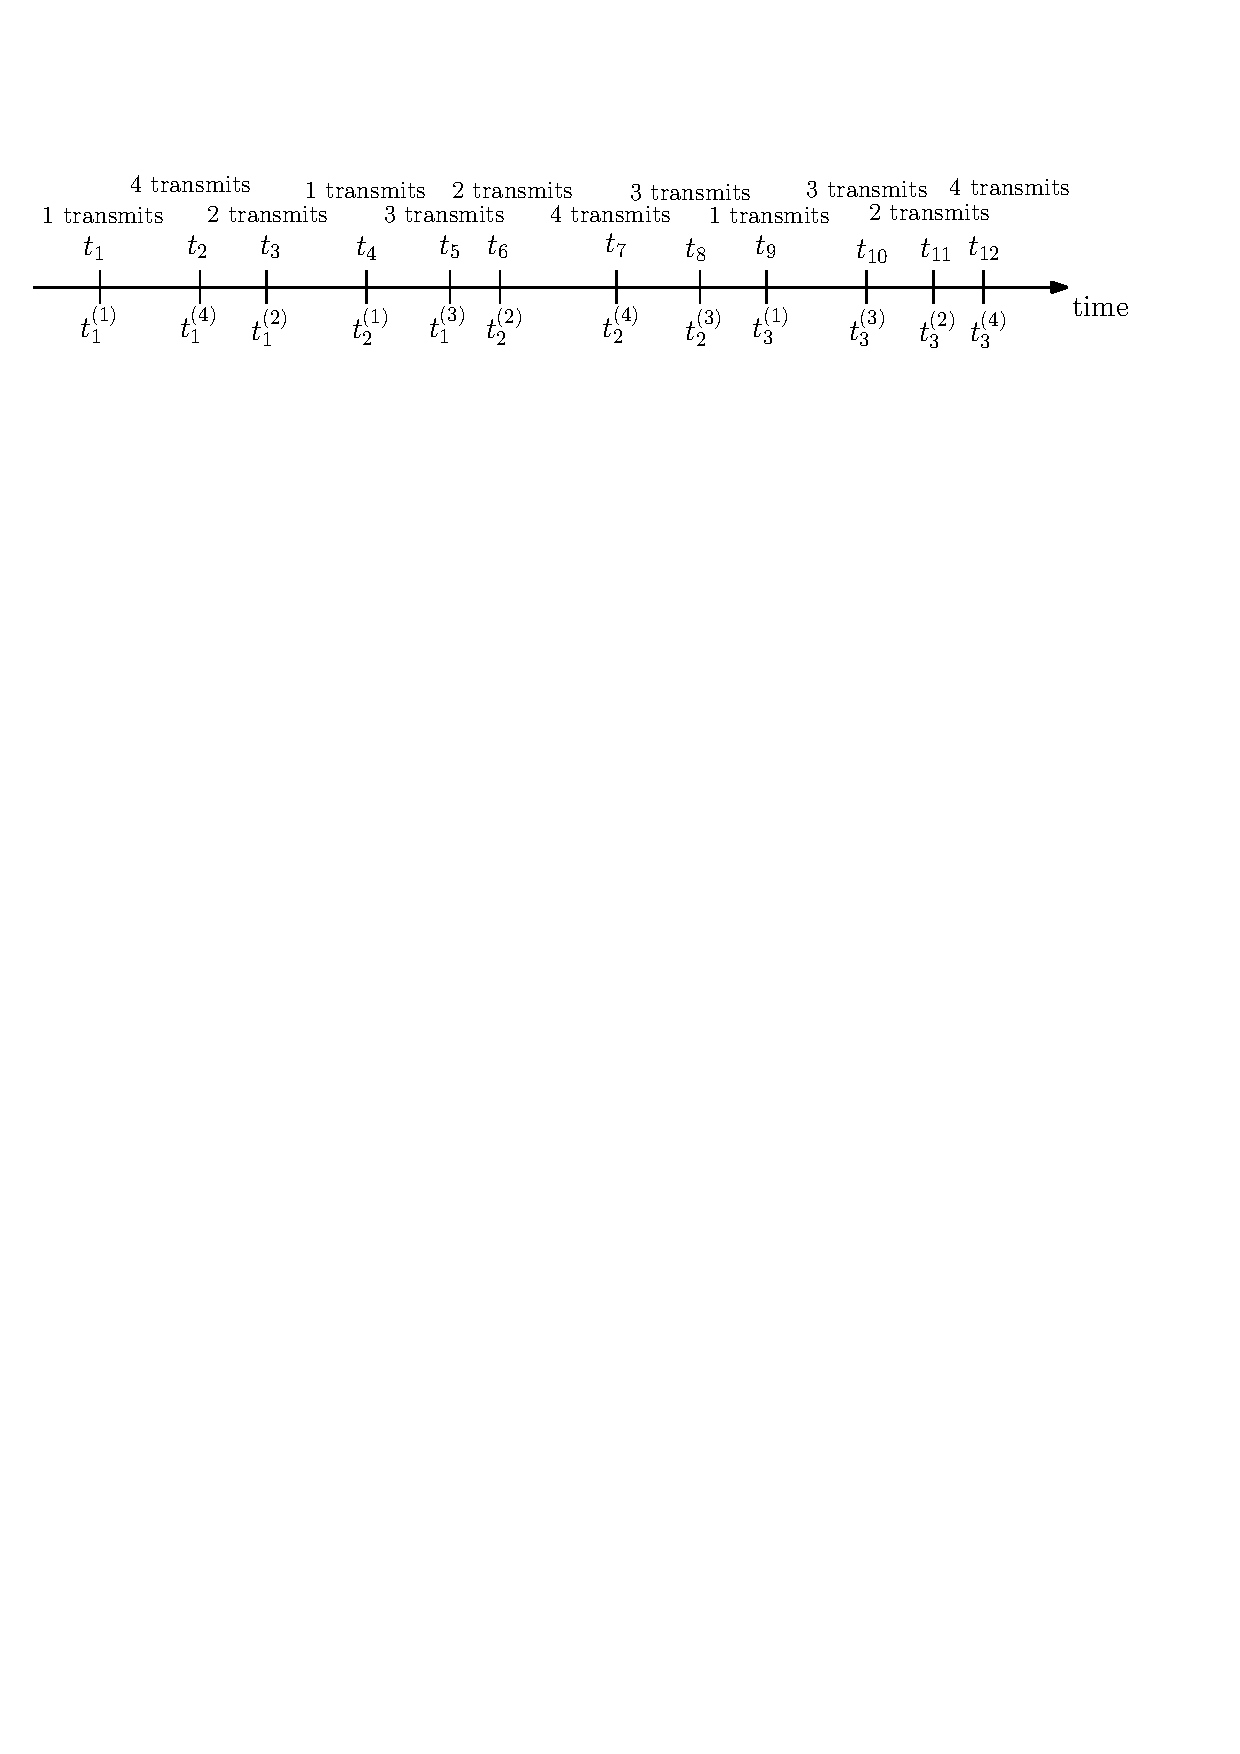
\includegraphics[width=0.9\textwidth]{timeline}
\end{center}






\section*{Appendix B -- Broadcast gossip average consensus}

This section is a reminder of some theoretical results about broadcast-gossip average-consensus algorithm.

Throughout this paragraph, we consider the discrete-time dynamics obtained by considering only the values of the state at the times $t_1, t_2, t_3 \dots$ as described in Appendix A, i.e., $x(k) := x(t_k)$. \\

The state update is $x(k+1) = P(k) x(k)$, with $P(k)$ a random matrix. Matrices $P(k)$ (for $k=0,1,2,\dots$) are i.i.d., uniformly extracted in a finite set of matrices $P^{(1)}, \dots, P^{(n)}$,  where a matrix $P^{(i)}$ corresponds to a node $i$ being extracted (i.e., transmitting) and the averaging update being done by $i$'s neighbors.\\


For given initial values $x(0)$, the trajectories of $x(k)$  will be random, depending on the random sequence in which nodes are activated to communicate. The expected value $\bar x(k) := \mathbb E x(k)$ will have the dynamics $\bar x(k+1) = \bar P \bar x(k)$, where $\bar P := \mathbb E P(k)$ (the expected value is the same for all $k$, since $P(k)$' s are identically distributed).
%Compute $\bar P$ (hint: $\bar P = \sum_{i=1}^n \frac{1}{n} P^{(i)}$);
%try to find a neat expression for $\bar P$, involving the Adjacency or the Laplacian matrix of the graph, and of course also the parameter $\alpha$.

Notice that $\bar P$ is a weighted adjacency matrix of the graph describing neighbors.

Also notice that the dynamics of $\bar x(k)$ are not random, this is the same as standard synchronous consensus, so that we can apply such a theory to study convergence of $\bar x(k)$.\\



%; if the graph is rooted (contains a rooted spanning tree), theory predicts convergence of all entries $\bar x(k)$ to a consensus value $\bar \pi^T x(0)$, where  $\bar \pi^T$ is the left dominant eigenvector of $\bar P$, namely $\bar \pi^T \bar P = \pi^T$ and $\sum_i \bar \pi_i = 1$. Look at $\bar P$: what can you say about $\bar \pi^T$? What can you say about the consensus value, in the case where the graph is undirected and connected?



It is important to notice that even if we can prove that the expected value $\bar x(k)$ converges to consensus, this does not imply that the random trajectories $x(k)$ will converge.
We need a deeper theoretical result to study convergence of random trajectories. The following theorem ensures that, under suitable conditions, the random trajectories do converge with high probability to a consensus (i.e., a common value), but this value might not be the same as the one to which $\bar x(k)$ converges.

%	About convergence of random trajectories, the following theorem holds:\\
	\textit{Theorem~1 (\cite{gossip-converg-as}, Coroll.~3.2})\\
	Assume that:
		\begin{itemize}
		\item For all node $i$, $P_{ii}(k)>0$ almost surely,
		\item the graph associated with $\bar P$ is strongly connected.
		\end{itemize}
	Then, $x(k)$ achieves probabilistic consensus, i.e.:
		\begin{itemize}
		\item If the initial condition is already a consensus $x(0) = a \mathbf 1$ for some scalar $a$, then
		$x(k) = a \mathbf 1$ for all k;
		\item given any initial condition $x(0)$, there exists a scalar random variable $x_{\infty}$ (depending on the initial condition), such that $x(k)$ converges almost surely to $x_{\infty} \mathbf 1$.
		\end{itemize}
	\hfill $\square$ \\
%	Verify that the assumptions of this theorem are satisfied by the broadcast gossip consensus that we are considering.
%	 \item

	 Theorem~1 guarantees almost sure convergence to a common consensus value. However, in general the consensus value $x_{\infty}$ is a random variable: for given initial values, it can vary depending on the random sequence $P(k)$ (i.e., depending on the random transmissions). For the broadcast gossip averaging algorithm, if the graph is undirected, in expectation we have $\bar P$ which is doubly-stochastic, so that the expectation $\bar x(k)$ will converge to average consensus, but each random realization $x(k)$ needs not to do so. The following theorem guarantees that the error between the random final value $x_{\infty}$ and the correct expected final value $\frac{1}{n}\sum_i x_i(0)$ cannot be too bad, there is an ensured upper bound for it, described below \textit{[read it, for your information, but you will not need this for the report]}.

	 Denote by $\bar x(k) :=  \mathbb E x(k)$ the expectation of the state, and denote by $x_{\text{ave}}(k) := \frac{1}{n}\sum_i x_i(k)$ the scalar random value obtained as the average of the states $x_i(k)$ at a given time $k$; notice that $x_{\text{ave}}(0)$ is not random, and is the desired average of the initial values.
	 Define $V(0) = \frac{1}{n} \sum_i (x_i(0) - x_{\text{ave}}(0))^2 $; this is a measure of dispersion of the initial values (it is natural to expect that the smaller $V(0)$ is, the easier it is to go to average consensus, since initial values are already near to it). Define $\gamma:= \frac{\alpha}{1-\alpha} d_{\max}$,
	 where $\alpha$ is the parameter used in the averaging broadcast gossip update and $d_{\max}$ is the maximum of the out-degrees of all nodes (out-degree being the number of neighbors to which a node can broadcast).

	\textit{Theorem~2 (\cite{gossip-small-error}, Theorem~1 and Example~2)}\\
For the averaging broadcast gossip algorithm and with the above definitions, the following bound holds true:
\[ \mathbb E [ (x_{\text{ave}}(k) - x_{\text{ave}}(0))^2 ] \le
 \frac{\gamma}{n} V(0)  \, .\]
If the graph associated with $\bar P$ is strongly connected, then Theorem~1 ensures that
$x(k)$ converges almost surely to $x_{\infty} \mathbf 1$ for some random variable $x_{\infty}$ and $\bar x(k)$ converges to $x_{\text{ave}}(0) \mathbf 1$;  the random variable $x_{\infty}$ satisfies the following bound:
\[ \mathbb E [ (x_{\infty} - x_{\text{ave}}(0))^2 ] \le
\frac{\gamma}{n} V(0)\,. \vspace{-2mm}\]
\hfill $\square$
%
%
%	\end{itemize}



\begin{thebibliography}{99}

\bibitem{consensus-tutorial}
F. Garin and L. Schenato, A survey on distributed estimation and control applications using linear consensus algorithms, in {\it Networked Control Systems}, A. Bemporad, M. Heemels, and M. Johansson eds, Springer LNCIS, vol.~406, Chapter~3, pp.~75--107, Springer, 2011, Available on-line: \url{http://necs.inrialpes.fr/people/garin/WIDEbook_GarinSchenato.pdf}


\bibitem{gossip-poisson}
S. Boyd, A. Ghosh, B. Prabhakar, and D. Shah, Randomized gossip algorithms, {\it IEEE Trans.\ on Information Theory}, vol.~52, no.~6, 2006, pp.~2508--2530, Available on-line: \url{http://web.mit.edu/devavrat/www/rand-gossip.pdf}


\bibitem{gossip-converg-as}
F. Fagnani and S. Zampieri, Randomized consensus algorithms over large scale networks,
{\it IEEE Journal on Selected Areas in Communications}, vol.~26, no.~4, 2008, pp.~634-–649, Available on-line:
\url{http://calvino.polito.it/~fagnani/coordincontrol/Random%20consensus.pdf}

\bibitem{gossip-small-error}
P. Frasca and J. M. Hendrickx, On the mean square error of randomized averaging algorithms, {\it Automatica}, vol.~49, no.~8, 2013, pp.~2496--2501, Available on-line: \url{http://arxiv.org/pdf/1111.4572.pdf}

\bibitem{RandSync-journal}
S. Bolognani, R. Carli, E. Lovisari, and S. Zampieri,
A randomized linear algorithm for clock synchronization in multi-agent systems,
to appear, {\it IEEE Trans.\ on Automatic Control}, vol.~61, no.~7, 2016.
Preprint available on-line:
\url{http://control.ee.ethz.ch/~bsaverio/papers/randsync.pdf}


\end{thebibliography}




\end{document}
